%======================================================================
\section{Geometry of growth and the dichotomy}\label{sec:geo}
%======================================================================

Corollary~\ref{cor:geo} turns the deficit into a counting problem: count the sites of $\Abar$ born farther from the cut than the reach $v(T-t_x)$ of the cone. The fractions below are those of a cone whose normal speed is exactly $v$, as for the brickwork pattern; for an arbitrary circuit of speed at most $v$ they are \emph{lower bounds} on the fraction never reached. We write $\lambda=v/s$ for the ratio of the causal speed to the speed of the front. Figure~\ref{fig:cone} summarises the geometry.

\begin{figure}[t]
\centering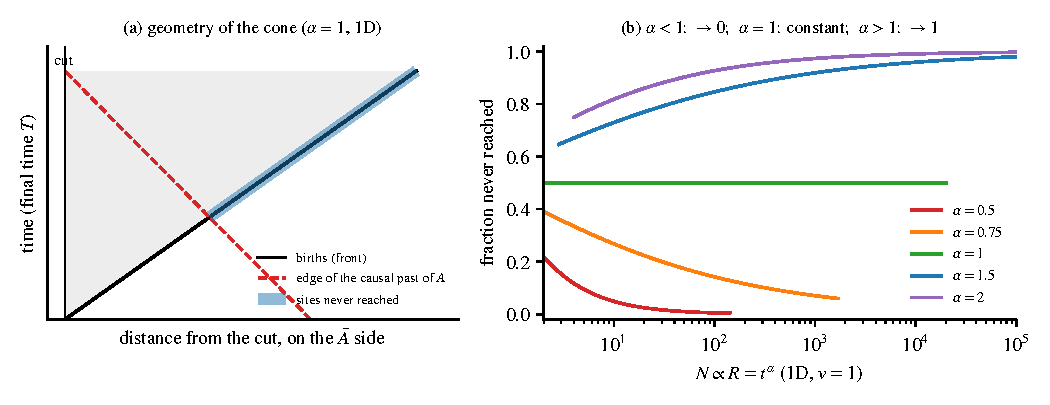
\includegraphics[width=\textwidth]{figures/fig_cone_geometry.pdf}
\caption{(a)~Geometry in one dimension for a linear front. A site is never reached (blue) if it is born beyond the edge of the causal past of the cut. (b)~Fraction of $\Abar$ out of reach as a function of size, for a front $R=t^\alpha$ and a causal speed $v=1$. It tends to $0$ if $\alpha<1$, stays constant (here $1/(1+v)$) if $\alpha=1$, and tends to $1$ if $\alpha>1$.}
\label{fig:cone}
\end{figure}

\begin{proposition}[front at constant speed, dimension $d$]\label{prop:front}
Consider a ball of radius $R(t)=st$ cut by a diametral hyperplane, and a cone of normal speed $v$. The fraction of $\Abar$ out of reach of the cone tends to
\begin{equation}\label{eq:fd}
f_d(\lambda)=\Big\langle 1-\Big(\frac{\lambda}{\lambda+u}\Big)^{d}\Big\rangle_{u},
\end{equation}
where $u$ is the direction cosine with respect to the normal, averaged over the hemisphere. One has $f_1=\frac{1}{1+\lambda}$, $f_3=1-\frac{\lambda(2\lambda+1)}{2(\lambda+1)^2}$ and $f_2=\frac1\pi\int_{-\pi/2}^{\pi/2}\big[1-\big(\frac{\lambda}{\lambda+\cos\theta}\big)^2\big]\dd\theta$. For every finite $\lambda$, $0<f_d(\lambda)<1$, and $f_d(\lambda)\sim d\langle u\rangle/\lambda$ as $\lambda\to\infty$.
\end{proposition}
\begin{proof}
A site at distance $r$ from the centre, with direction cosine $u>0$, is born at $t_x=r/s$. It is out of reach if and only if $ru>v(T-r/s)=\lambda(R-r)$, that is $r>\lambda R/(\lambda+u)$ (Coq lemmas \texttt{front\_not\_reached} and \texttt{front\_threshold}). In direction $u$, the fraction of volume beyond this radius is $1-(\lambda/(\lambda+u))^d$.
\end{proof}

In one dimension, with a birth at the edge every $k$ layers ($s=1/k$, $v=1$), $f_1=1/(1+k)$ and hence $G\ge\frac{N}{2}\frac{\log q}{1+k}-O(1)$. This is the absence of a threshold: the deficit stays extensive for every finite $k$.

\begin{remark}[Eden--Richardson model]\label{rem:eden}
In this model \cite{Eden1961,Richardson1973}, every empty site adjacent to the cluster is born at a constant rate $r>0$. The shape theorem \cite{Richardson1973,CoxDurrett1981} states that the cluster grows linearly with a convex limit shape. The birth times therefore satisfy $t_x=\mu(x)(1+o(1))$ for a norm $\mu$ invariant under the symmetries of the lattice, including the reflection through the cut, and a non-zero fraction of sites is out of reach, the analogue of \eqref{eq:fd} for the norm $\mu$. The shape theorem is used as a black box.
\end{remark}

\begin{proposition}[constant global rate]\label{prop:rate}
If sites are born at rate $\gamma$ per unit time inside a growing ball, so that $N=\gamma t$ and $R\propto t^{1/d}$, the number of sites of $\Abar$ out of reach is
\begin{equation}\label{eq:rate}
\#\{x\in\Abar:\ \mathrm d_\perp(x,A)>v(T-t_x)\}\simeq\frac{\gamma\,\omega_{d-1}}{d\,\omega_d\,v}\,R\;\propto\;N^{1/d},
\end{equation}
where $\omega_k$ is the volume of the unit ball in dimension $k$ (for $d=2$: $\gamma R/(\pi v)$). This number is extensive for $d=1$ and sub-extensive for $d\ge2$.
\end{proposition}
\begin{proof}
One has $\dot R=\gamma/(d\,\omega_dR^{d-1})$. A site at depth $\delta$ below the edge, at distance $\rho=Ru$ from the cut, was born a time $\delta/\dot R$ ago; it is out of reach if $\delta<\rho\dot R/v$. Integrate over the hemisphere of the edge, with $\int_{u>0}u\,\dd\Omega=\omega_{d-1}$.
\end{proof}

\begin{estimate}[homogeneous 1D expansion, continuum approximation]\label{est:homog}
Sites are inserted at uniformly random positions following a law $N(t)$. Assume that the comoving coordinate $u\in[0,1]$ of a site stays fixed (in reality it fluctuates as in a P\'olya urn). The cut is at $u=\frac12$ and the cone has speed $v$ in sites per unit time. A site born when the system had $N_b$ sites is out of reach if $u-\frac12>\Delta(N_b)=\int_{t_b}^Tv\,\dd t/N(t)$, and the fraction of $\Abar$ out of reach is $f=\frac{1}{N_T}\int\dd N_b\,(1-2\Delta)_+$. With $\tau=cN_0/v$:
\begin{itemize}[leftmargin=*,itemsep=1pt]
\item if $N=N_0(1+t/\tau)^{p}$ with $p<1$, then $\Delta\to\infty$ and $f\to0$;
\item if $p=1$, then $\Delta=c\ln(N_T/N_b)$ and $f=1-2c\,(1-e^{-1/(2c)})\in(0,1)$ (Coq lemmas \texttt{fraction\_p1\_pos} and \texttt{fraction\_p1\_lt1});
\item if $p>1$, then $\Delta\to0$ and $f\to1$; for exponential growth, about $v\tau\,[\ln(N_T/2v\tau)+O(1)]$ sites of $\Abar$ are reached.
\end{itemize}
\end{estimate}

The cases $p>1$ and exponential admit a simpler rigorous bound. Insertion preserves the order of the sites, so the sites of $A$ (the final left half) always form a prefix of the chain, and a single link separates $A$ from $\Abar$. A two-qudit gate across the cut increases $S(A)$ by at most $2\log q$. Hence $S(A)\le2\log q$ times the number of layers, that is $S(A)=O(N^{1/p})$ for $p>1$ and $S(A)\le2\tau\ln(N/N_0)\log q$ for exponential growth. The latter case is a random MERA run in the direction of growth: the $O(\log N)$ bound is Vidal's causal-cone bound \cite{Vidal2007,Vidal2008}, and the MERA has the causal structure of a discrete de Sitter space \cite{Beny2013,BaoDS2017}.

\begin{proposition}[sub-volume scaling laws]\label{prop:scaling}
Consider a circuit with $v$ layers per unit time and a region $A$ bounded by a planar cut of section $|\partial A(t)|\propto L(t)^{d-1}$. For a linear size $L\propto t^\alpha$ with $\alpha>1$,
\begin{equation}\label{eq:scaling}
S(A)\le C\,N^{\,1-\frac{\alpha-1}{\alpha d}} .
\end{equation}
For exponential growth ($L\propto e^{Ht}$), $S(A)\le C\,(v/H)\,L^{d-1}$ if $d\ge2$ (\emph{area law}) and $S(A)\le C\,(v/H)\ln L$ if $d=1$.
\end{proposition}
\begin{proof}
Every gate across the cut increases $S(A)$ by at most $2\log q$, and a layer contains at most $|\partial A(t)|$ such gates. Hence $S(A)\le2\log q\,v\int_0^T|\partial A(t)|\,\dd t\propto T^{\alpha(d-1)+1}$, while $N\propto T^{\alpha d}$. For a Hamiltonian, the entangling-rate bound of \cite{VanAcoleyen2013,Marien2016} gives the same result.
\end{proof}

Proposition~\ref{prop:scaling} follows directly from known area-times-time bounds and does not use the cone. For $\alpha\le1$ the same bound only gives $O(N)$, with no useful coefficient. It is in the marginal case $\alpha=1$ that the cone (Proposition~\ref{prop:front}) supplies the decisive information: a coefficient strictly below the maximum.

\begin{theoremL}\label{thm:C}
Consider isotropic front growth on $\mathbb Z^d$: a ball of radius $R(t)\propto t^\alpha$ cut by a diametral hyperplane, with growth symmetric under the reflection through this hyperplane (births in mirror pairs).
\begin{enumerate}[label=(\alph*),leftmargin=*]
\item If $\alpha\ge1$, then $G\ge c\,N-o(N)$ with $c>0$ for \emph{every} circuit of finite causal speed $v$ and, by Theorem~B, for every Lieb--Robinson dynamics on a fixed graph. One has $c=\frac12f_d(v/s)\log q$ for $\alpha=1$ and $c=\frac12\log q$ for $\alpha>1$.
\item If $\alpha<1$, there is a circuit of nearest-neighbour two-qudit gates, with $k$ layers per unit time ($k$ finite), such that $G=O(N\,T^{\alpha-1}/k)=o(N)$ at every time $T$.
\end{enumerate}
\end{theoremL}

\begin{proof}[Proof of (a); (b) is proven in Appendix~\ref{app:C}]
For $\alpha=1$, combine Corollary~\ref{cor:geo} and Proposition~\ref{prop:front}. For $\alpha>1$, Proposition~\ref{prop:scaling} gives $S=o(N)$. By symmetry, $|A|=|\Abar|$.
\end{proof}

The construction of (b) is a ``rainbow'' circuit \cite{Vitagliano2010}: in every row normal to the cut, newborn mirror pairs are brought side by side by an odd--even transposition sort, entangled into Bell pairs, and sent back; every Bell pair then straddles the cut. Only the sites born during the last cycle are unpaired, and a cycle lasts $O(R/k)$, a vanishing fraction of the age $T$ when $\alpha<1$.

\begin{remark}[extension normal to the cut]\label{rem:slab}
The criterion is about the extension \emph{normal} to the cut, not about linear size in general. Take a slab of fixed thickness $W$ that grows linearly parallel to the cut: $L\propto t$, but every site is within $W/2$ of the cut, and construction~(b), with rows of length at most $W$, gives $G=O(NW/(kT))=o(N)$.
\end{remark}

\begin{remark}[what a ``local growth rule'' means]\label{rem:local}
\begin{itemize}[leftmargin=*,itemsep=1pt]
\item \emph{Eden--Richardson}: $\alpha=1$, and the deficit is extensive for every local dynamics, in every dimension (Remark~\ref{rem:eden}).
\item \emph{Constant global rate}: $\alpha=1/d$, and the deficit is not guaranteed for $d\ge2$ (Theorem~C(b), Proposition~\ref{prop:rate}). Such a rate requires global coordination, or a single active site as in spiral growth.
\item \emph{Decelerated homogeneous expansion} ($N\propto t^p$, $p<1$, $d=1$): Estimate~\ref{est:homog} indicates that the cone catches up with everything; Theorem~A only guarantees an $O(1)$ deficit.
\end{itemize}
\end{remark}
